\documentclass{article}
\usepackage[T2A]{fontenc}
\usepackage[utf8]{inputenc}
\usepackage{graphicx}
\usepackage[export]{adjustbox}
\usepackage{geometry}
\usepackage{float}
\usepackage{indentfirst}

\graphicspath{ {./img/} }

\geometry{verbose,a4paper,tmargin=2cm,bmargin=2cm,lmargin=2.5cm,rmargin=1.5cm}

% \overfullrule=2cm
\newcommand{\paragraphline}[1]{\paragraph{#1}\mbox{}\\}

\title{Cartesian closed categories and the price of eggs}
\author{Вычиков Дмитрий}
\date{13.03.2019}
\begin{document}
    \maketitle
    \section{Актеры}
    \begin{enumerate}
        \item Администратор (Преподаватель) - пользователь, которые имеет права на создание и редактирование тестовых шаблонов, а также может создавать тестовые события и назначать их группам студентов.
        \item Пользователь (Студент или Преподаватель) - пользователь, которые имеет права на прохождение назначенных ему событий и просмотр результатов.
    \end{enumerate}
    
    % \textbf{}

    % \paragraph{Создать/Редактировать тестовый шаблон}
    \section{Варианты использования}
    \subsection{Создать/Редактировать тестовый шаблон}
    \textbf{Описание:} Администратор изменяет существующий тестовый шаблон\\
    \textbf{Предусловия:}Тестовый шаблон создан\\
    \textbf{Основной поток событий:}
    \begin{enumerate}
        \item Администратор открывает страницу создания/редактирования шаблона
        \item Администратор изменяет имя шаблона
        \item Если Администратор желает Добавить/Редактировать тестовый вопрос, выполняется вариант использования Добавить/Редактировать тестовый вопрос.
        \item Если Администратор желает удалить тестовый вопрос, выполняется вариант использования Удалить вопрос.
        \item Вариант использования завершается
        \item Администратор сохраняет шаблон
    \end{enumerate} 
    
    \subsection{Добавить тестовый вопрос}
    \textbf{Описание:} Администратор добавляет новый вопрос в тестовый шаблон\\
    \textbf{Предусловия:} Тестовый шаблон создан\\
    \textbf{Основной поток событий:}
    \begin{enumerate}
        \item Администратор добавляет пустой тестовый вопрос
        \item Администратор задает текст вопроса
        \item Если Администратор желает задать сигнатуру тестовой процедуры, выполняется вариант использования Задать вид тестовой процедуры.
        \item Если Администратор желает добавить верное решение решение в виде процедуры, выполняется вариант использования Задать верное решение.
        \item Если Администратор желает задать набор входных тестовых данных , выполняется вариант использования Задать входные данные для тестирования
        \item Вариант использования завершается
    \end{enumerate}


    \subsection{Задать вид тестовой процедуры}
    \textbf{Описание:} Администратор создает объект процедуры, описывающей вид входных и выходных данных\\
    \textbf{Предусловия:} Тестовый вопрос создан\\
    \textbf{Основной поток событий:}
    \begin{enumerate}
        \item Администратор задает название процедуры в соответствующем поле
        \item Администратор выбирает тип возвращаемого процедурой значения из списка допустимых значений.
        \item Администратор задает набор входных параметров
        \item Вариант использования завершается
        \item Задать верное решение
    \end{enumerate}
    
    \subsection{Задать верное решение}
    \textbf{Описание:} Администратор задает код процедуры, который решает
    поставленную в вопросе задачу и выдает результаты, с которыми впоследствии
    будут сравниваться результаты, полученные от пользовательского кода\\
    \textbf{Предусловия:} Тестовый процедура создана\\
    \textbf{Основной поток событий:}
    \begin{enumerate}
        \item Администратор записывает код процедуры в соответствующем поле
        \item Вариант использования завершается
    \end{enumerate}

    \subsection{Задать входные данные для тестирования}
    \textbf{Описание:} Администратор задает наборы значений всех входных аргументов для тестируемой функции\\
    \textbf{Предусловия:} Тестовый процедура создана\\
    \textbf{Основной поток событий:}
    \begin{enumerate}
        \item Администратор записывает наборы входных данных в определенном в формате в соответствующее поле
        \item Вариант использования завершается
    \end{enumerate}
    
    \subsection{Просмотреть список шаблонов}
    \textbf{Описание:} Администратор просматривает список существующих тестовых
    шаблонов, доступных для редактирования или создания события\\
    \textbf{Предусловия:} Нет\\
    \textbf{Основной поток событий:}
    \begin{enumerate}
        \item Администратор записывает наборы входных данных в определенном в формате в соответствующее поле
        \item Вариант использования завершается
    \end{enumerate}

    
    \subsection{Создать тестовое событие}
    \textbf{Описание:} Администратор создает тестовое событие на основе одного
    из шаблонов и задает список студентов, которые должны пройти это событие.\\
    \textbf{Предусловия:} Существует хотя бы один тестовый шаблон.\\
    \textbf{Основной поток событий:}
    \begin{enumerate}
        \item Если Администратор желает задать время начала/окончания события, выполняется вариант использования Задать дату и время начала/окончания события.
        \item Если Администратор желает выбрать тестовый шаблон для события, выполняется вариант использования Выбрать тестовый шаблон.
        \item Если Администратор желает задать список студентов, которым необходимо пройти тестовое событие, выполняется вариант использования Указать список тестируемых студентов
        \item Администратор нажимает кнопку “Создать”
        \item Вариант использования завершается
    \end{enumerate}


    \subsection{Задать дату и время начала/окончания события}
    \textbf{Описание:} Администратор задает временной промежуток, в течение
    которого пользователям будет доступно это событие.\\
    \textbf{Предусловия:} Выполняется вариант использования Создать тестовое
    событие.\\
    \textbf{Основной поток событий:}
    \begin{enumerate}
        \item Администратор выбирает дату и время начала и окончания события на интерфейсе
        \item Вариант использования завершается
    \end{enumerate}


    \subsection{Выбрать тестовый шаблон}
    \textbf{Описание:} Администратор выбирает один из существующих тестовых
    шаблонов, который будет использован при проведении события.\\
    \textbf{Предусловия:}
    \begin{enumerate}
       \item Существует хотя бы один тестовый шаблон
       \item Выполняется вариант использования “Создать тестовое событие”
    \end{enumerate}
    \textbf{Основной поток событий:}
    \begin{enumerate}
        \item Администратор выбирает тестовый шаблон из предоставленного списка
        \item Администратор нажимает кнопку “Подтвердить”
        \item Вариант использования завершается    
    \end{enumerate}


    \subsection{Указать список тестируемых студентов}
    \textbf{Описание:} Администратор выбирает студентов, которым
    необходимо пройти это тестовое событие\\
    \textbf{Предусловия:} Выполняется вариант использования “Создать
    тестовое событие”\\
    \textbf{Основной поток событий:}
    \begin{enumerate}
        \item Администратор выбирает студентов/группы студентов из списка
        \item Вариант использования завершается
    \end{enumerate}


    \subsection{Просмотреть список доступных тестовых событий}
    \textbf{Описание:} Пользователь просматривает список событий, которые были на него назначены\\
    \textbf{Предусловия:} Нет\\
    \textbf{Основной поток событий:}
    \begin{enumerate}
        \item Пользователь открывает страницу со списком доступных событий
        \item Вариант использования завершается
    \end{enumerate}


    \subsection{Запустить тестовое событие}
    \textbf{Описание:} Пользователь начинает одно из назначенных ему тестовых
    событий\\
    \textbf{Предусловия:} 
    \begin{enumerate}
        \item Пользователь имеет назначенные на него события
        \item Событие уже стало доступно и еще не закончилось
    \end{enumerate}
    \textbf{Основной поток событий:}
    \begin{enumerate}
        \item Пользователь выбирает событие и нажимает кнопку “Начать”.
        \item Пользователь вводит ответы на вопросы теста.
        \item Если пользователь желает проверить правильность своего решения, выполняется вариант использования Запросить проверку решения.
        \item Пользователь нажимает кнопку “Завершить”
        \item Вариант использования завершается    
    \end{enumerate}

    \subsection{Запросить проверку решения}
    \textbf{Описание:} Пользователь запрашивает проверку своего решения для вопроса\\
    \textbf{Предусловия:} Выполняется вариант использования “Запустить тестовое событие”\\
    \textbf{Основной поток событий:}
    \begin{enumerate}
        \item Пользователь нажимает кнопку “Проверить решение” и через некоторое время получает результат проверки
        \item Вариант использования завершается
    \end{enumerate}

    \subsection{Просмотреть результаты пройденных тестов}
    \textbf{Описание:} Пользователь просматривает историю своих пройденных событий\\
    \textbf{Предусловия:} Нет\\
    \textbf{Основной поток событий:}
    \begin{enumerate}
        \item Пользователь переходит на страницу с результатами пройденных тестов
        \item Вариант использования завершается
    \end{enumerate}

    \section{Диаграммы классов и пакетов}
    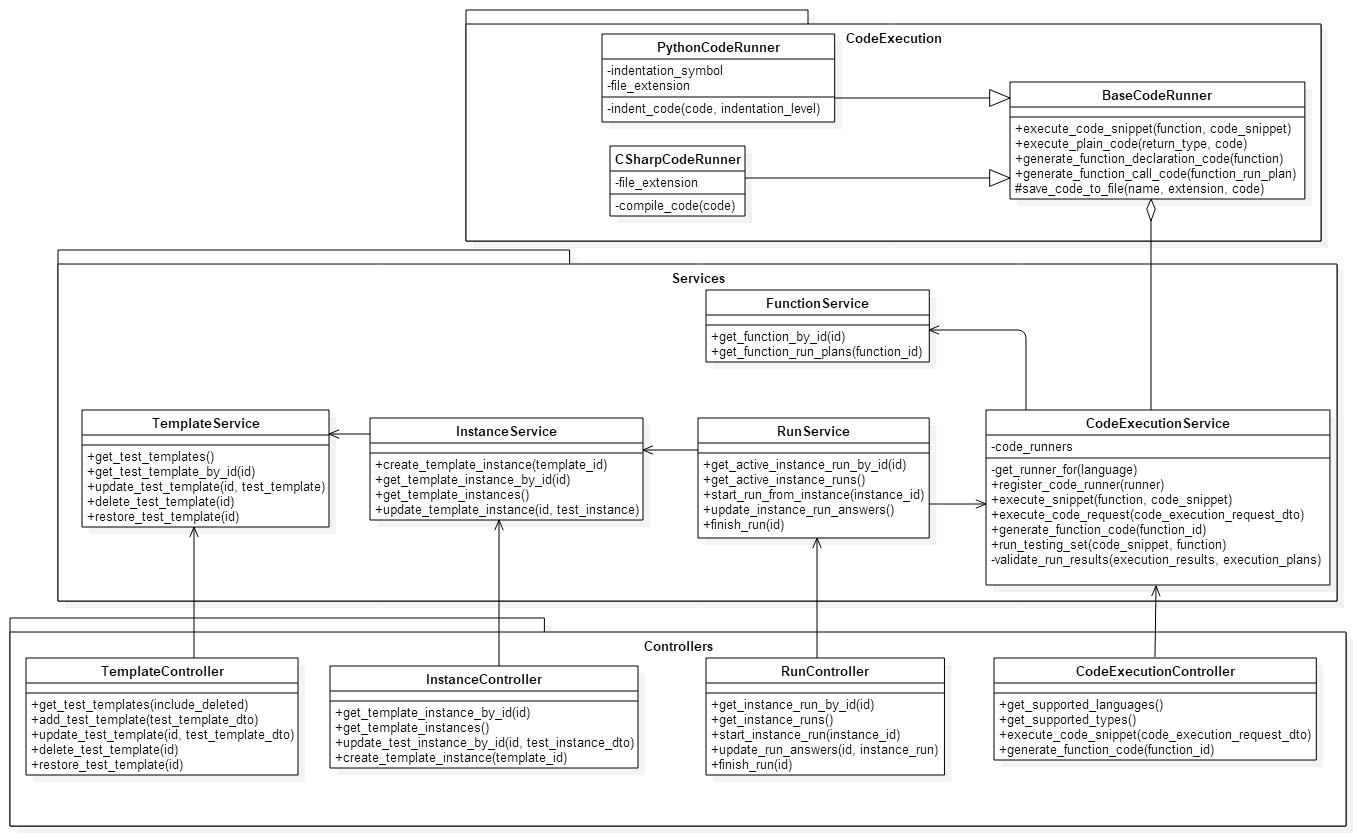
\includegraphics[width=\textwidth, keepaspectratio, angle=270,center]
    {ClassDiagram_Services}
    \pagebreak

    \subsection{} Пакет \textbf{Controllers} содержит классы-контроллеры, определяющие набор публичных REST-эндпоинтов, с которыми может взаимодествовать клиент.\par
    Контроллеры сами не содержат никакой бизнес-логики, а лишь перенаправляют вызовы к бизнес-слою (сервисам) и возвращают результат клиенту.    \begin{enumerate}
        \item TemplateController - отвечает за создание, редактирование, удаление тестовых шаблонов
        \item InstanceController - отвечает за создание тестовых событий из шаблонов
        \item RunController - позволяет запускать тестовые события, вносить в них изменения и завершать.
        \item CodeExecutionController - позволяет получить список доступных языков и типов, а также провести запуск какого-либо кода
    \end{enumerate}
    \parПакет \textbf{Services} содержит объекты сервисы, с которыми взаимодействуют контроллеры.
    Сервисы реализуют бизнес операции, которые позволяют совершать контроллеры.
    \parИх зона ответственности совпадает с зоной ответственности одноименных контроллеров, поэтому 
    данное описание будет опущено.
    \begin{enumerate}
        \item TemplateService
        \item InstanceService
        \item RunService
        \item CodeExecutionService
    \end{enumerate}
    \par
    Пакет \textbf{CodeExecution} содержит классы, которые реализуют логику предварительной подготовки исполняемого кода и взаимодействием с окружением, непосредственно на котором этот код будет запускаться.
    \begin{enumerate}
        \item BaseCodeRunner - базовый класс "исполнителей" кода, который определяет набор абстрактных
        операций, необходимых для подготовки и запуска кода. Реализация этих операций будет находиться в классах-наследниках.
        \item PythonCodeRunner - класс для взаимодействия с окружением языка Python
        \item CSharpCodeRunner - класс для взаимодействия с окружением языка C\#
    \end{enumerate}
    
    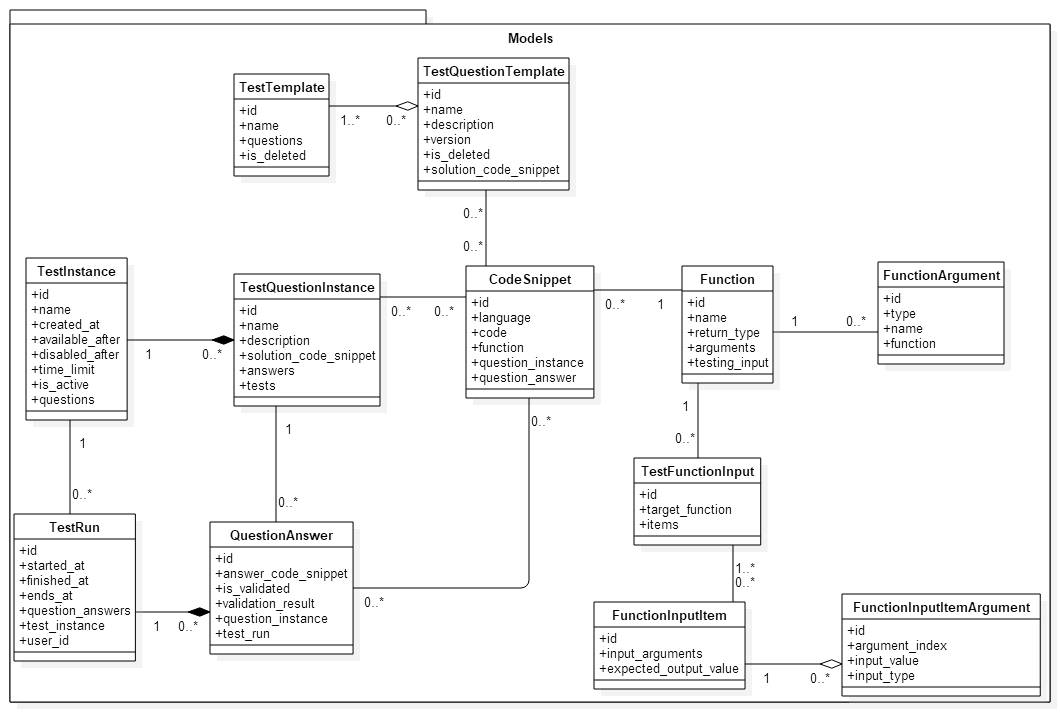
\includegraphics[width=\textwidth, keepaspectratio, center]{ClassDiagram_Models}

    \par Пакет \textbf{Models} содержит классы моделей, которые отражают предметную область и являются объектами,
    хранящими данные системы. Конфигурация таблиц базы данных соответствует моделям данных, что достигается
    при помощи использовании технологий ORM - Object Relational Mapping.
    \begin{enumerate}
        \item TestTemplate - Тестовый шаблон. Содержит имя шаблона и список входящих 
        в него вопросов.
        \item TestQuestionTemplate - Шаблон вопроса. Содержит имя, описание,
        номер версии и ссылку на код процедуры правильного решения.
        \item CodeSnippet - Объект представляющий код процедуры. Содержит
        идентификатор языка, на котором написан код, сам код, а также ссылку
        на объект функции.
        \item Function - Представляет сигнатуру исполняемой функции. Содержит
        следующие поля: имя, тип возвращаемого значения, список аргементов и
        набор входных данных для тестирования.
        \item Function Argument - Аргумент функции. Имеет имя и тип.
        \item TestFunctionInput - Набор данных для тестирования. Имеет ссылку на
        тестируемую функцию и список входных данных.
        \item FunctionInputItem - Описывает конкретные значения входных и выходных
        параметров теста
        \item FunctionInputItemArgument - Описает тип и значение конкретного аргумента
        функции
        \item TestInstance - Тестовое событие. Содержит название, дату и время начала
        и окончания события, а также список вопросов.
        \item TestQuestionInstance - Вопрос тестового события. Дублирует поля
        объекта TestQuestionTemplate, но также хранит список ответов, данных
        на этот вопрос.
        \item TestRun - Предствляет процедуру проведения тестирования.
        Содержит следующие поля: дату и время начала, планируемого окончания
        тестирования, фактического окончания тестирования, список данных ответов и
        ID пользователя, проходящего тестирование.
        \item QuestionAnswer - Ответ на вопрос. Содежит ссылку на фрагмент кода
        решения, результат проверки и флаг, показывающий, был ли этот вопрос
        проверен или еще нет.
    \end{enumerate}

    \section{Диаграммы последовательностей и кооперации}
    

    \subsection{Создать/Редактировать тестовый шаблон}   
        \begin{figure}[H]
            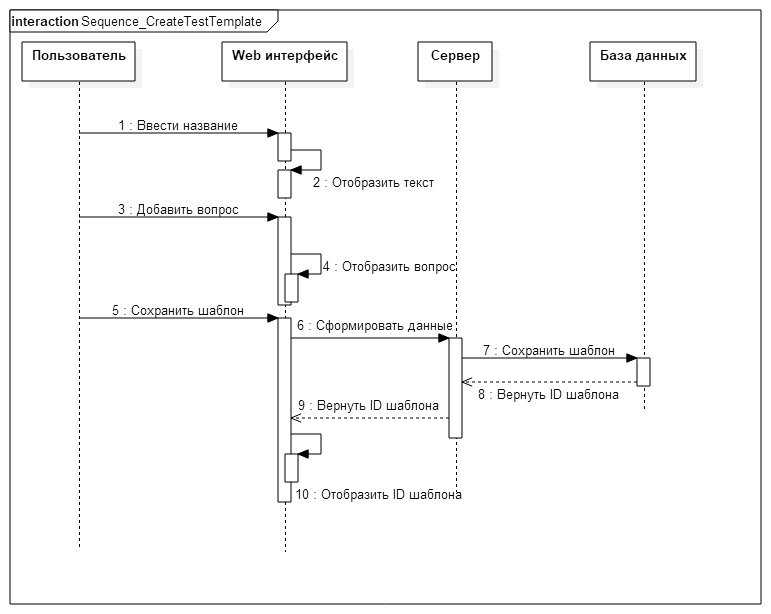
\includegraphics[width=\textwidth, center]{Sequence_CreateTestTemplate}
            \caption{Диаграмма последовательности}
        \end{figure}
        
        \paragraph{Объекты:}
        \begin{enumerate}
            \item Пользователь
            \item WEB-интерфейс
            \item Сервер
            \item База данных
        \end{enumerate}
        
        \paragraph{Сообщения между объектами:}
        \begin{enumerate}
            \item Ввести название
            \item Отобразить текст
            \item Добавить вопрос
            \item Добавить Отобразить вопрос
            \item Сохранить шаблон
            \item Сформировать данные
            \item Сохранить шаблон
            \item Вернуть ID шаблона
            \item Вернуть ID шаблона
            \item Отобразить ID шаблона
        \end{enumerate}
        \paragraph{}
        Пользователь формирует шаблон при помощи WEB-интерфейс, после чего тот
        отправляет сформированный шаблон на сервер для сохранения в базе данных

        \begin{figure}[H]
            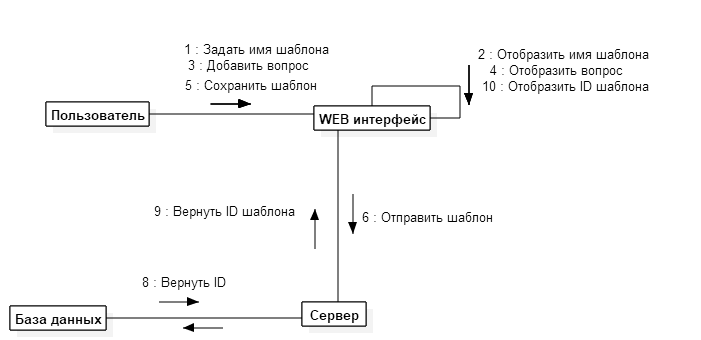
\includegraphics[width=\textwidth, center]{Communication_CreateTestTemplate}
            \caption{Диаграмма кооперации}
        \end{figure}
        \paragraph{}
        Диаграмма кооперации отражает те же объекты и процессы, что и диаграмма
        последовательности.


    \subsection{Добавить тестовый вопрос}
        \begin{figure}[H]
            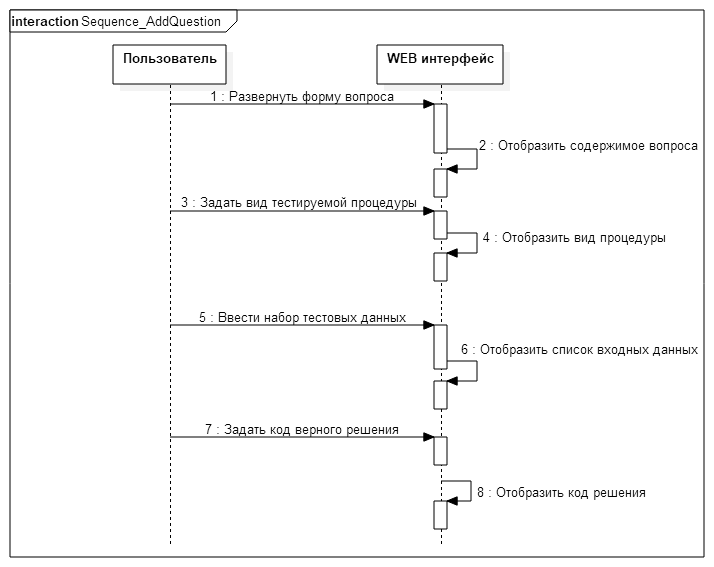
\includegraphics[width=\textwidth, center]{Sequence_AddQuestion}
            \caption{Диаграмма последовательности}
        \end{figure}
        \paragraph{Объекты:}
        \begin{enumerate}
            \item Пользователь
            \item WEB-интерфейс
        \end{enumerate}
        \paragraph{Сообщения между объектами:}
        \begin{enumerate}
            \item Развернуть форму вопроса
            \item Отобразить содержимое вопроса
            \item Задать вид тестируемой процедуры
            \item Отобразить вид процедуры        
            \item Ввести набор тестовых данных        
        \end{enumerate}
        \paragraph{}
        Пользователь задает вид тестовой функции, вводит набор входных данных
        для тестирования и, если требуется, предоставляет код верного решения задачи.
        \begin{figure}[H]
            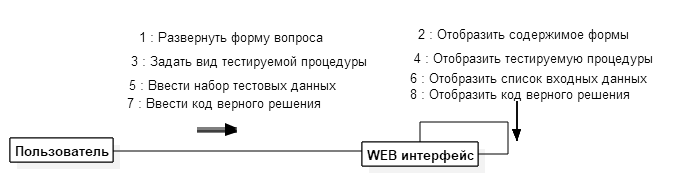
\includegraphics[width=\textwidth, center]{Communication_AddQuestion}
            \caption{Диаграмма кооперации}
        \end{figure}
        \paragraph{}
        Диаграмма кооперации отражает те же объекты и процессы, что и диаграмма
        последовательности.


    \subsection{Задать вид тестируемой процедуры}
        \begin{figure}[H]
            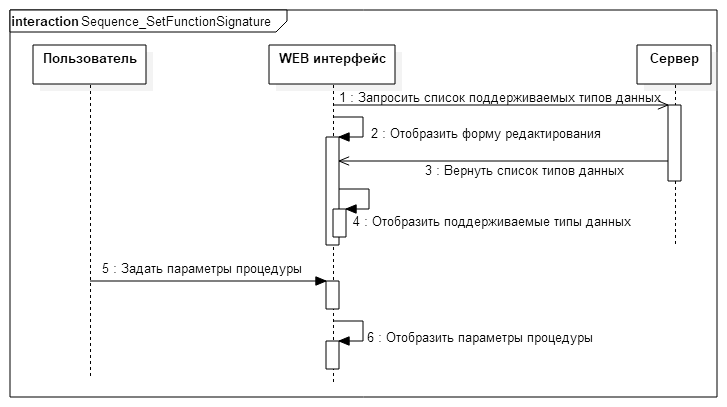
\includegraphics[width=\textwidth, center]
                {Sequence_SetFunctionSignature}
            \caption{Диаграмма последовательности}
        \end{figure}
        \paragraph{Объекты:}
        \begin{enumerate}
            \item Пользователь
            \item WEB-интерфейс
            \item Сервер
        \end{enumerate}
        \paragraph{Сообщения между объектами:}
        \begin{enumerate}
            \item Запросить список поддерживаемые типов данных
            \item Отобразить форму редактирования
            \item Вернуть список типов данных
            \item Отобразить поддерживаемые типы данных
            \item Задать параметры процедуры
            \item Отобразить параметры процедуры
        \end{enumerate}
        \paragraph{}
        WEB клиент запрашивает у сервера список поддерживаемых типов данных.
        После ответа сервера пользователь задает имя тестируемой процедуры,
        тип возвращаемого значения, а также имена и типы аргументов.
        \begin{figure}[H]
            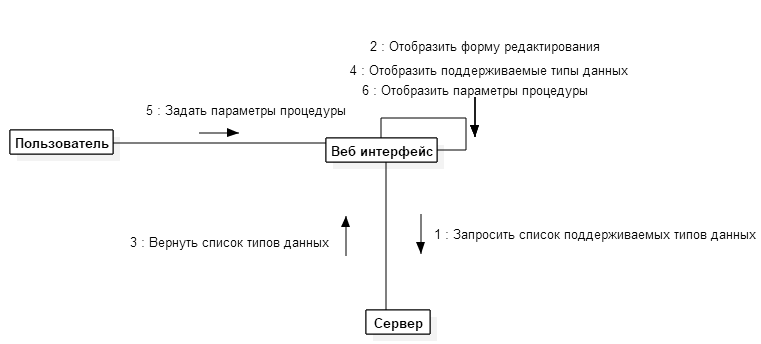
\includegraphics[width=\textwidth, center]
                {Communication_SetFunctionSignature}
            \caption{Диаграмма кооперации}
        \end{figure}
        \paragraph{}
        Диаграмма кооперации отражает те же объекты и процессы, что и диаграмма
        последовательности.


    \subsection{Задать верное решение}
        \begin{figure}[H]
            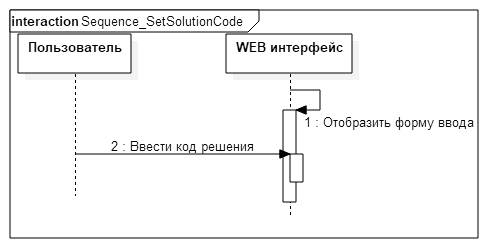
\includegraphics[width=\textwidth, center]
                {Sequence_SetSolutionCode}
            \caption{Диаграмма последовательности}
        \end{figure}
        \paragraph{Объекты:}
        \begin{enumerate}
            \item Пользователь
            \item WEB-интерфейс
        \end{enumerate}
        \paragraph{Сообщения между объектами:}
        \begin{enumerate}
            \item Отобразить форму ввода
            \item Ввести код решения
        \end{enumerate}
        \paragraph{}
        Пользователь вводит код своего решения в форму на WEB интерфейсе
        \begin{figure}[H]
            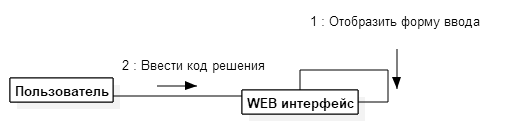
\includegraphics[width=\textwidth, center]
                {Communication_SetSolutionCode}
            \caption{Диаграмма кооперации}
        \end{figure}
        \paragraph{}
        Диаграмма кооперации отражает те же объекты и процессы, что и диаграмма
        последовательности.
    
    \subsection{Задать входные данные для тестирования}
        \begin{figure}[H]
            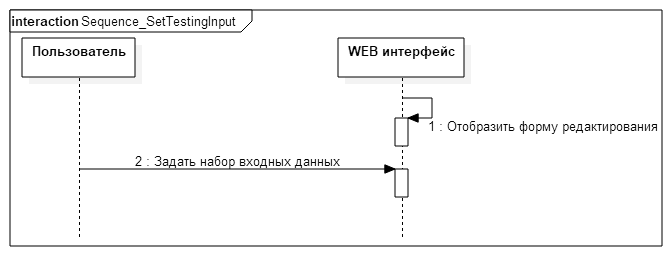
\includegraphics[width=\textwidth, center]
                {Sequence_SetTestingInput}
            \caption{Диаграмма последовательности}
        \end{figure}
        \paragraph{Объекты:}
        \begin{enumerate}
            \item Пользователь
            \item WEB-интерфейс
        \end{enumerate}
        \paragraph{Сообщения между объектами:}
        \begin{enumerate}
            \item Отобразить форму редактирования
            \item Задать набор входных данных
        \end{enumerate}
        \paragraph{}
        Пользователь вводит набор тестовых даннных в определенном формате
        в соответствующую форму на WEB интерфейсе
        \begin{figure}[H]
            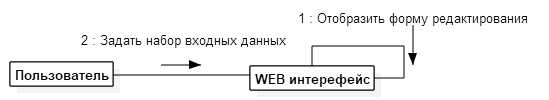
\includegraphics[width=\textwidth, center]
                {Communication_SetTestingInput}
            \caption{Диаграмма кооперации}
        \end{figure}
        \paragraph{}
        Диаграмма кооперации отражает те же объекты и процессы, что и диаграмма
        последовательности.
    
    
    \subsection{Создать тестовое событие}
        \begin{figure}[H]
            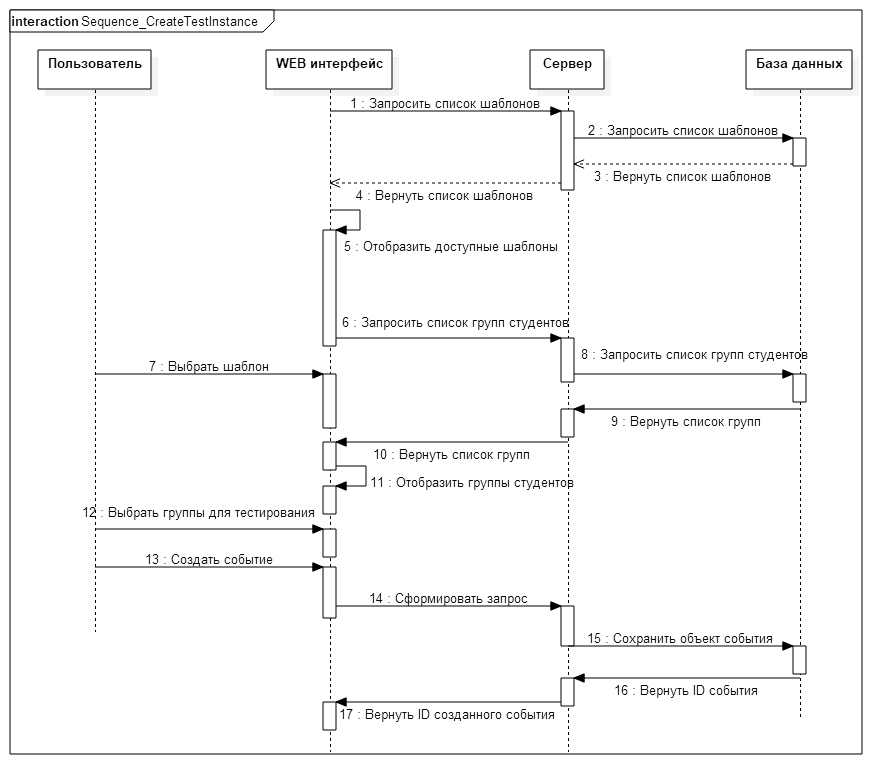
\includegraphics[width=\textwidth, center]
                {Sequence_CreateTestInstance}
            \caption{Диаграмма последовательности}
        \end{figure}
        \paragraph{Объекты:}
        \begin{enumerate}
            \item Пользователь
            \item WEB-интерфейс
            \item Сервер
            \item База данных
        \end{enumerate}
        \paragraph{Сообщения между объектами:}
        \begin{enumerate}
            \item Запросить список шаблонов
            \item Запросить список шаблонов
            \item Вернуть список шаблонов
            \item Вернуть список шаблонов
            \item Отобразить доступные шаблоны
            \item Запросить список групп студентов
            \item Запросить список групп студентов
            \item Вернуть список групп
            \item Вернуть список групп
            \item Отобразить группы студентов
            \item Выбрать группы для тестирования
            \item Создать событие
            \item Сформировать запрос
            \item Сохранить объект события
            \item Вернуть ID события
            \item Вернуть созданного ID события
        \end{enumerate}
        \paragraph{}
        WEB-клиент запрашивает у сервера список доступных шаблонов и группы
        студентов. После чего пользователь выбирает нужный шаблон из списка,
        выбирает студентов для прохождения тестирования и создает событие.
        \begin{figure}[H]
            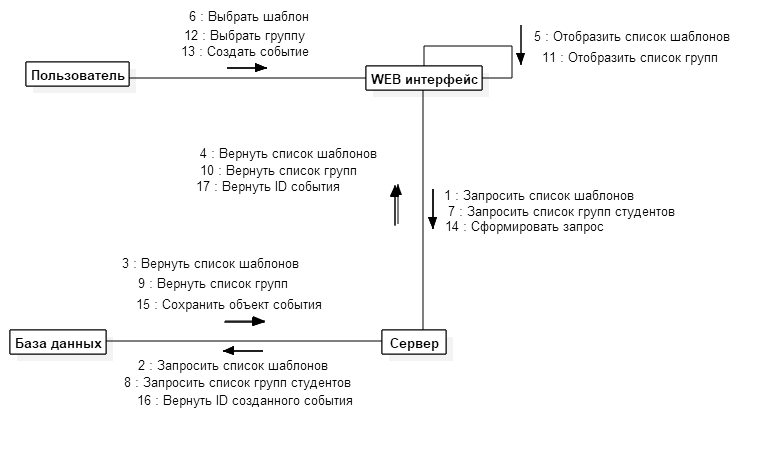
\includegraphics[width=\textwidth, center]
                {Communication_CreateTestInstance}
            \caption{Диаграмма кооперации}
        \end{figure}
        \paragraph{}
        Диаграмма кооперации отражает те же объекты и процессы, что и диаграмма
        последовательности.
    
    
    \subsection{Просмотреть список шаблонов}
        \begin{figure}[H]
            \includegraphics[width=\textwidth, center]
                {Sequence_ViewTemplatesList}
            \caption{Диаграмма последовательности}
        \end{figure}
        \paragraph{Объекты:}
        \begin{enumerate}
            \item Пользователь
            \item WEB-интерфейс
            \item Сервер
            \item База данных
        \end{enumerate}
        \paragraph{Сообщения между объектами:}
        \begin{enumerate}
            \item Открыть страницу шаблонов
            \item Запросить список шаблонов
            \item Вернуть список шаблонов
            \item Вернуть список шаблонов
            \item Отобразить список шаблонов
        \end{enumerate}
        \paragraph{}
        WEB-клиент запрашивает у сервера список доступных шаблонов для просмотра.
        \begin{figure}[H]
            \includegraphics[width=\textwidth, center]
                {Communication_ViewTemplatesList}
            \caption{Диаграмма кооперации}
        \end{figure}
        \paragraph{}
        Диаграмма кооперации отражает те же объекты и процессы, что и диаграмма
        последовательности.
    
    
    \subsection{Запустить тестовое событие}
        \begin{figure}[H]
            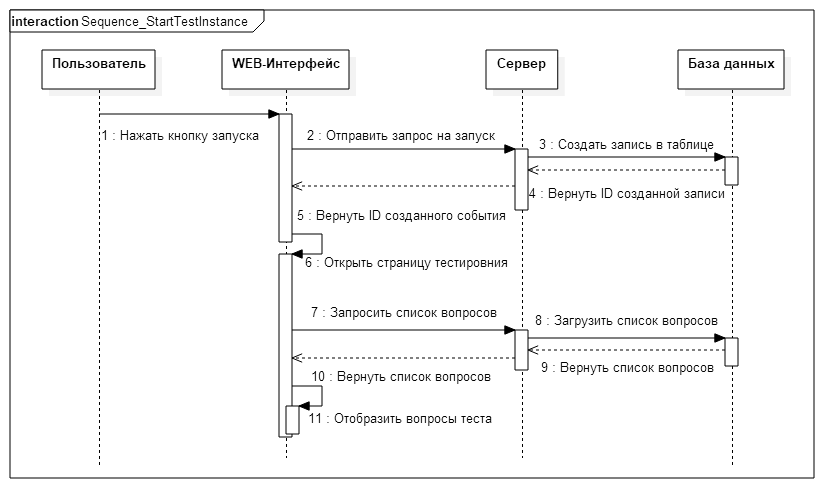
\includegraphics[width=\textwidth, center]
                {Sequence_StartTestInstance}
            \caption{Диаграмма последовательности}
        \end{figure}
        \paragraph{Объекты:}
        \begin{enumerate}
            \item Пользователь
            \item WEB-интерфейс
            \item Сервер
            \item База данных
        \end{enumerate}
        \paragraph{Сообщения между объектами:}
        \begin{enumerate}
            \item Нажать кнопку запуска
            \item Отправить запрос на запуск
            \item Создать запись в таблцие
            \item Вернуть ID созданной записи
            \item Вернуть ID созданного события
            \item Открыть страницу тестирования
            \item Запросить список вопросов
            \item Загрузить список вопросов
            \item Вернуть список вопросов
            \item Вернуть список вопросов
            \item Отобразить вопросы теста
        \end{enumerate}
        \paragraph{}
        Пользователь нажимает на кнопку запуска событие. WEB-клиент посылает
        соответствующий запрос на сервер и, получив ответ, открывает страницу
        прохождения тестирования и загружает список вопросов.
        \begin{figure}[H]
            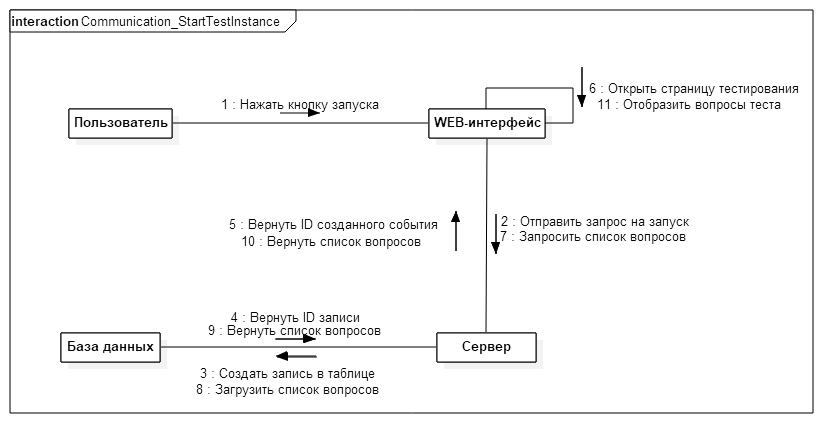
\includegraphics[width=\textwidth, center]
                {Communication_StartTestInstance}
            \caption{Диаграмма кооперации}
        \end{figure}
        \paragraph{}
        Диаграмма кооперации отражает те же объекты и процессы, что и диаграмма
        последовательности.
    
    
    \subsection{Запросить проверку решения}
        \begin{figure}[H]
            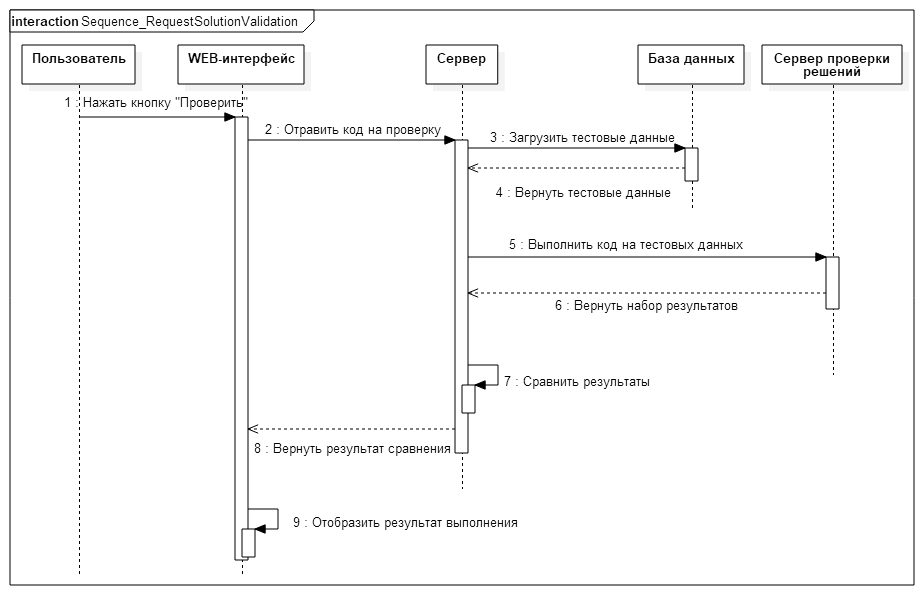
\includegraphics[width=\textwidth, center]
                {Sequence_RequestSolutionValidation}
            \caption{Диаграмма последовательности}
        \end{figure}
        \paragraph{Объекты:}
        \begin{enumerate}
            \item Пользователь
            \item WEB-интерфейс
            \item Сервер
            \item База данных
        \end{enumerate}
        \paragraph{Сообщения между объектами:}
        \begin{enumerate}
            \item Нажать кнопку "Проверить"
            \item Отравить код на проверку
            \item Загрузить тестовые данные
            \item Вернуть тестовые данные
            \item Выполнить код на тестовых данных
            \item Вернуть набор результатов
            \item Сравнить результаты
            \item Отобразить результат выполнения
        \end{enumerate}
        \paragraph{}
        Пользователь запрашивает проверку своего решения. WEB-клиент отправляет
        тестируемый код на сервер. Сервер загружает из базы данных набор
        данных для тестирования и запускает код пользователя со всеми вариантами
        входных данных на сервере выполнения кода. После чего сравнивает ответы
        с ожидаемыми и возвращает клиенту.
        \begin{figure}[H]
            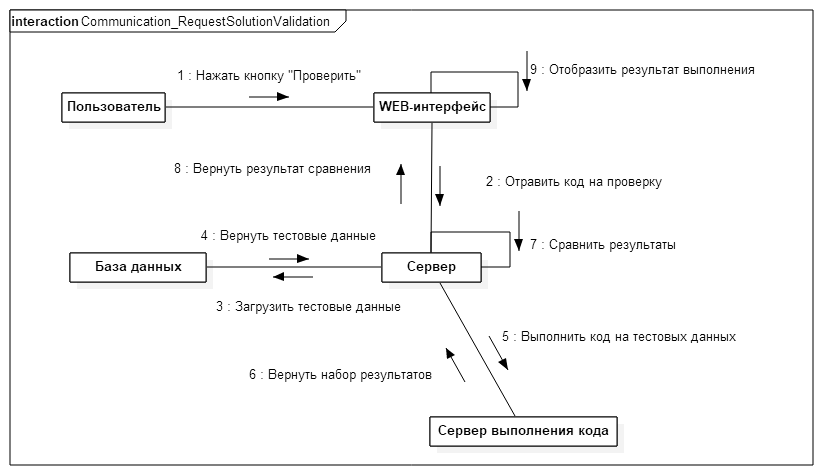
\includegraphics[width=\textwidth, center]
                {Communication_RequestSolutionValidation}
            \caption{Диаграмма кооперации}
        \end{figure}
        \paragraph{}
        Диаграмма кооперации отражает те же объекты и процессы, что и диаграмма
        последовательности.
    
    
    \subsection{Просмотреть результаты пройденных тестов}
        \begin{figure}[H]
            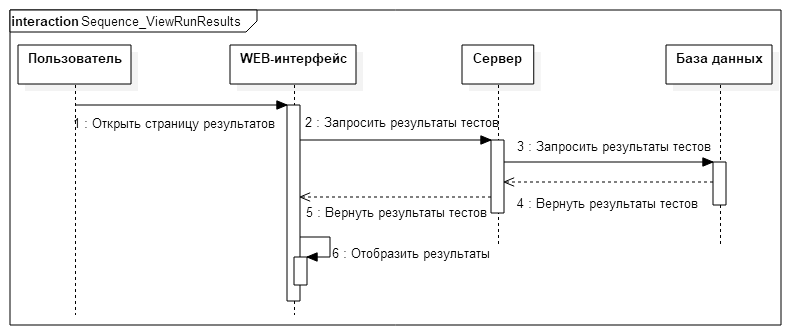
\includegraphics[width=\textwidth, center]
                {Sequence_ViewRunResults}
            \caption{Диаграмма последовательности}
        \end{figure}
        \paragraph{Объекты:}
        \begin{enumerate}
            \item Пользователь
            \item WEB-интерфейс
            \item Сервер
            \item База данных
        \end{enumerate}
        \paragraph{Сообщения между объектами:}
        \begin{enumerate}
            \item Нажать кнопку "Проверить"
            \item Отравить код на проверку
            \item Загрузить тестовые данные
            \item Вернуть тестовые данные
            \item Выполнить код на тестовых данных
            \item Вернуть набор результатов
            \item Сравнить результаты
            \item Отобразить результат выполнения
        \end{enumerate}
        \paragraph{}
        Пользователь открывает страницу просмотра результатов прохождения
        тестового события. WEB-клиент запрашивает данные у сервера, который
        загружает из базы данных и отображает на интерфейсе.
        \begin{figure}[H]
            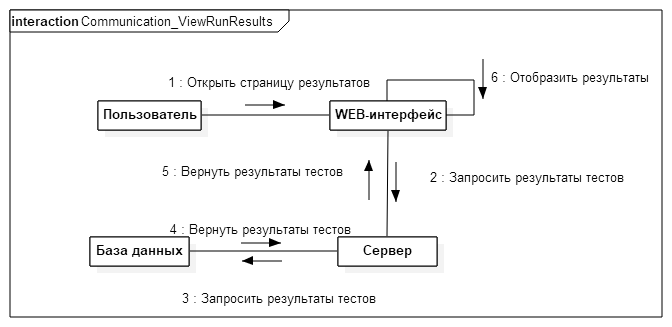
\includegraphics[width=\textwidth, center]
                {Communication_ViewRunResults}
            \caption{Диаграмма кооперации}
        \end{figure}
        \paragraph{}
        Диаграмма кооперации отражает те же объекты и процессы, что и диаграмма
        последовательности.
    
    
    
    
    \section{Диаграмма состояний}
    \begin{figure}[H]
        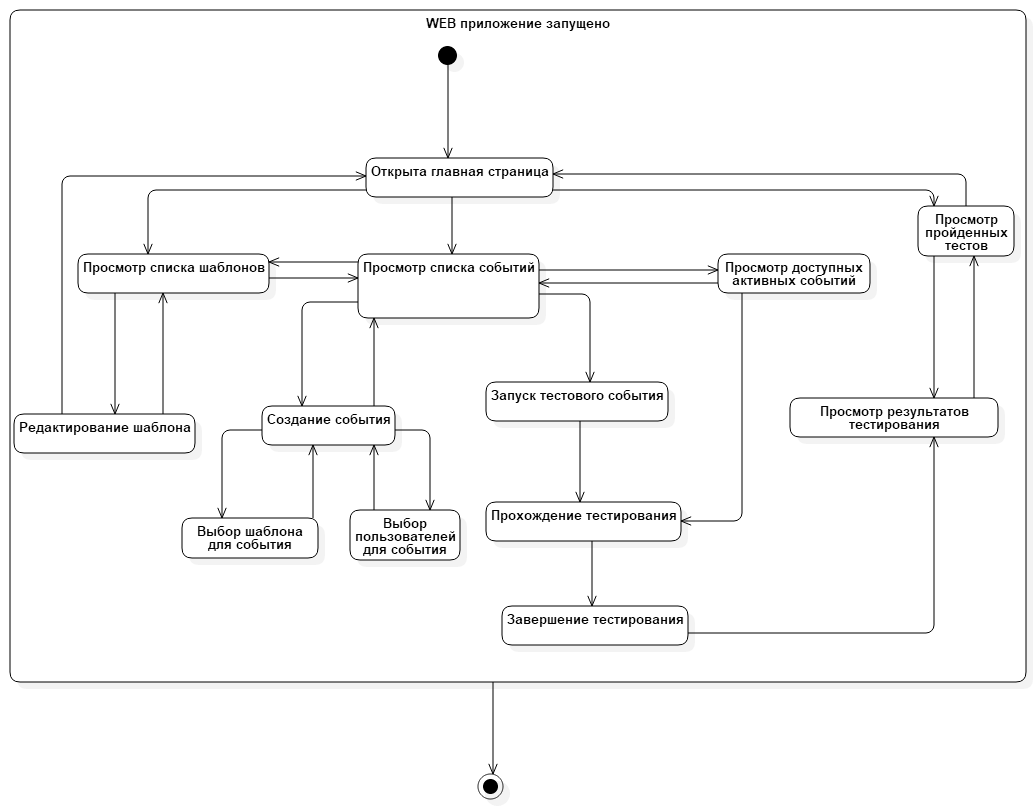
\includegraphics[width=\textwidth, center]{Statechart_WEB.png}        
        \caption{Диаграмма состояний}
    \end{figure}
    \paragraph{}
    При открытии WEB-страницы приложение находится в
    состоянии "Открыта главная страница". Отсюда можно перейти 
    в состояния  Просмотр списка шаблонов", "Просмотр списка событий",
    "Просмотр пройденных тестов".
    \par Из состояния "Просмотр списка шаблонов" можно перейти
    к редактированию одного из шаблонов.
    \par Из состояния "Просмотр событий" можно перейти в
    состояние "Создание события", если администратор хочет
    создать новое событие, или в состояние "Запуск тестового
    события", если он хочет запустить событие.
    \par Из состояния "Создание события" можно попасть в
    состояния "Выбор шаблона для события" и "Выбор пользователей"
    для события, или вернуться к просмотру списка событий.
    \par Из состояния "Запуск тестового события" пользователь
    попадает в состояние "Прохождение тестирования", а потом - 
    в состояние "Завершение тестирования". Также, можно
    продолжить прохождение тестирования, перейдя к нему из
    состояния "Просмотр доступных активных" событий.
    \par После завершения тестирования пользователь будет
    перенаправлен в состояние "Просмотр результатов тестирования".
    Также, узнать результаты пройденного теста можно, перейдя
    на соответствующую страницу из состояния "Просмотр пройденных
    тестов".
    \par Из любого состояния можно перейти на главную страницу
    или закончить работу с приложением. Эти переходы не отражены
    на диаграмме, чтобы не загромождать ее огромным количеством
    стрелок.

    
    \section{Диаграмма деятельности}
    \begin{figure}[H]
        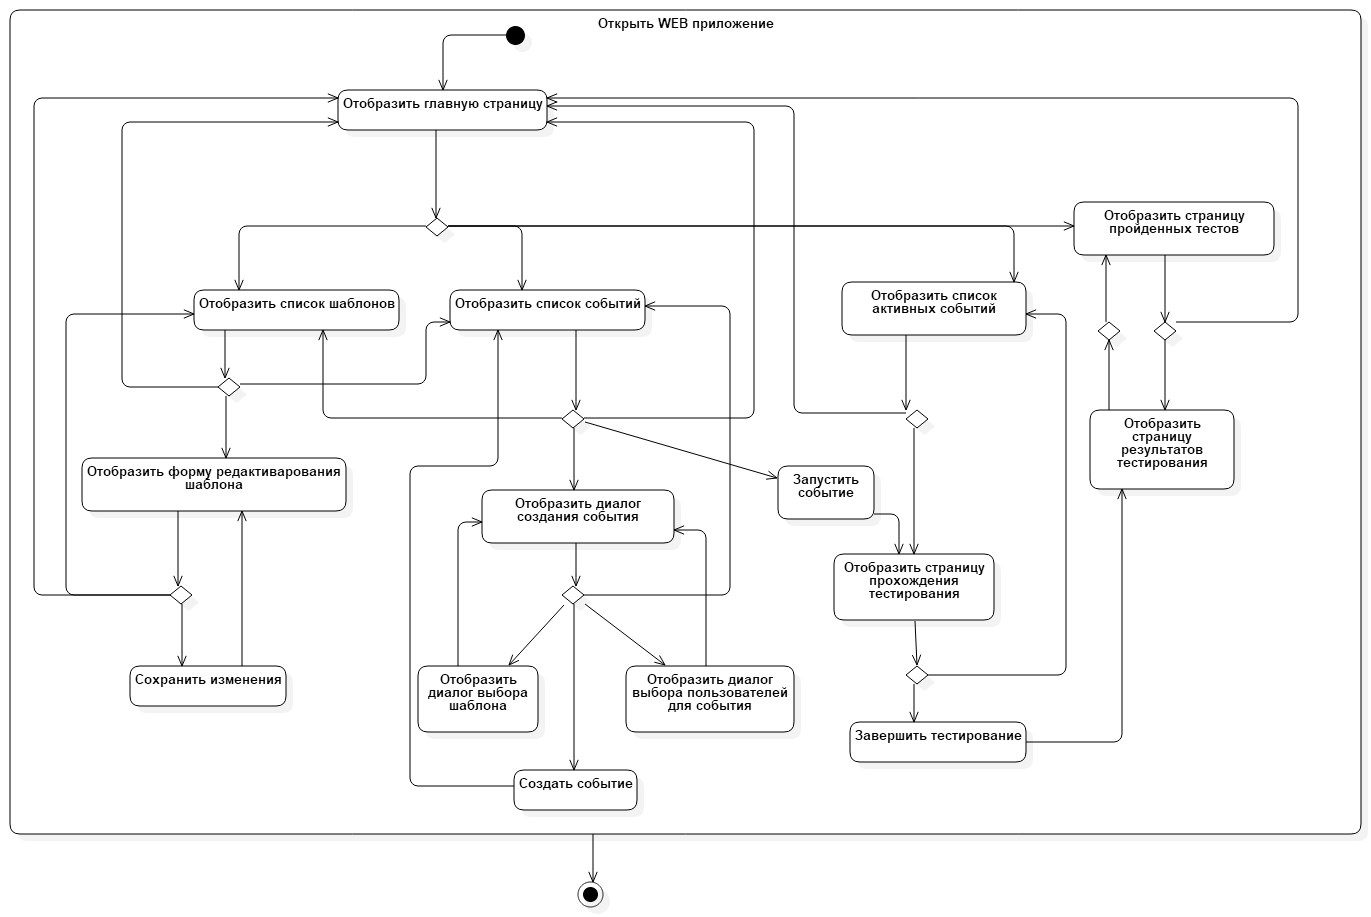
\includegraphics[width=\textwidth, center]
        {ActivityDiagram_WEB.png}
        \caption{Диаграмма деятельности}
    \end{figure}
        
    После отображения главной страницы пользватель может
    открыть страницы списка шаблонов, списка событий, списка
    пройденных тестов.

    При создании события есть возможность выбрать шаблон
    тестирования и список пользоватей, которым нужно пройти это
    тест.
    
    Запустив событие, пользователь будет перенаправлен
    на страницу прохождения тестирвоания, а помтом - на страницу
    результатов.
    
    На страницу результатов также можно попасть со страницы
    пройденных тестов.
    
    Если тестирование уже начато, то к нему можно вернуться
    со страницы со списком активных событий.
    \section{Диаграмма компонентов}
    \begin{figure}[H]
        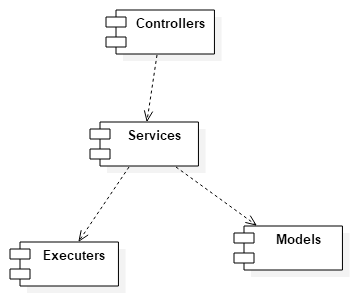
\includegraphics[width=\textwidth, center]
        {ComponentDiagram.png}
        \caption{Диаграмма компонентов}
    \end{figure}
    Система разделена на следующие компоненты:
    \begin{enumerate}
        \item Controllers - компонент, описывающий интерфейс
        взаимодействия с внешними системами
        \item Services - компонент, содержащий бизнес-логику
        приложения.
        \item Models - содержит описание моделей данных,
        использующихся в приложении
        \item Executers - компонент, который взаимодействует
        со сторонними серверами/контейнерами, осуществуляющими
        выполнение кода.
    \end{enumerate}
    
    
    \section{Диаграмма развертывания}
    \begin{figure}[H]
        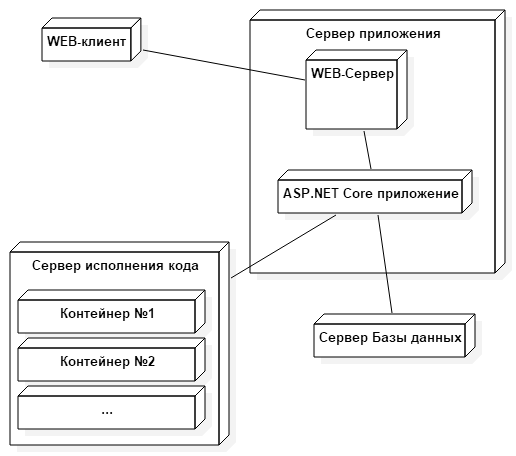
\includegraphics[width=\textwidth, center]
        {DeploymentDiagram.png}
        \caption{Диаграмма развертывания}
    \end{figure}
    Система состоит и четырех частей:
    \begin{enumerate}
        \item WEB-client (например, браузер пользователя)
        \item Application Server - сервер, на котором выполняется
        код главной части приложения.
        \item Database Server - сервер, на котором находится
        база данных
        \item CodeExecutionServer - сервер, на котором
        находятся изолированные контейнеры, внутри которых
        запускается и тестируется пользовательский код.
    \end{enumerate}
    
\end{document}
